%!TEX root = ../../tcc.tex

\subsection*{Uso do IPv6}

O IPv6 tem duas datas marcantes: o Dia Mundial e o Dia do Lançamento Mundial. O Dia
Mundial do IPv6, ou \emph{World IPv6 Day}, organizado pelo \emph{Internet Society}
(ISOC) \cite{site:isoc-ipv6day}, ocorreu no dia 8 de junho de 2011, e contou com a
participação de grandes empresas estrangeiras (Facebook, Google, Yahoo!, Akamai,
Lamelight Networks, etc) e brasileiras (Terra, Campus Party, IG), num teste de 24 horas
de oferecimento de conexão e conteúdo utilizando o protocolo IPv6. O evento foi
considerado um sucesso pela ISOC.

Já o Dia de Lançamento Mundial do IPv6, em dia 6 de junho de 2012, foi um evento
semelhante ao Dia Mundial, com o mesmo objetivo e com mais participantes, porém,
mantendo o IPv6 habilitado após o evento \cite{site:isoc-ipv6launch}. Desde então,
empresas do mundo todo têm corrido contra o relógio para que o oferecimento de conexões
de Internet não seja estagnado pela falta de endereços.

O IPv6 precisa ser suportado pelas pontas das redes (aplicações em clientes e
servidores) e pelas rotas entre eles (provedores de acesso, empresas de
telecomunicações). Enquanto o primeiro é simples, pois bastam configurações de
conectores dos respectivos sistemas operacionais, servidores de aplicação e roteadores
internos que suportem o IPv6, o caminhos entre ambos é mais complicado. Para as empresas
provedoras de acesso, envolve custos de troca de equipamentos de infraestrutura de
rede, além do treinamento da mão de obra. Por conta disso, a transição para o novo
protocolo ainda é complexa e lenta.

\newpage
A situação ainda está devagar no contexto brasileiro do IPv6. Segundo o SindiTelebrasil,
em novembro de 2013 \cite{site:ipv6brasil}, as operadoras brasileiras ainda estavam
adquirindo equipamentos. O cenário era considerado preocupante e, devido ao atraso da
migração tecnológica, medidas paliativas estão sendo tomadas.

Uma delas é o compartilhamento de endereços IPv4 por usuários, com restrição de portas,
o que pode afetar a experiência de uso de alguns tipos de aplicações. Esse
compartilhamento é feito numa estrutura com dois \glspl*{nat}, usando o modelo chamado
de \gls*{nat}444.

\begin{figure}[H]
    \centering
    \fbox{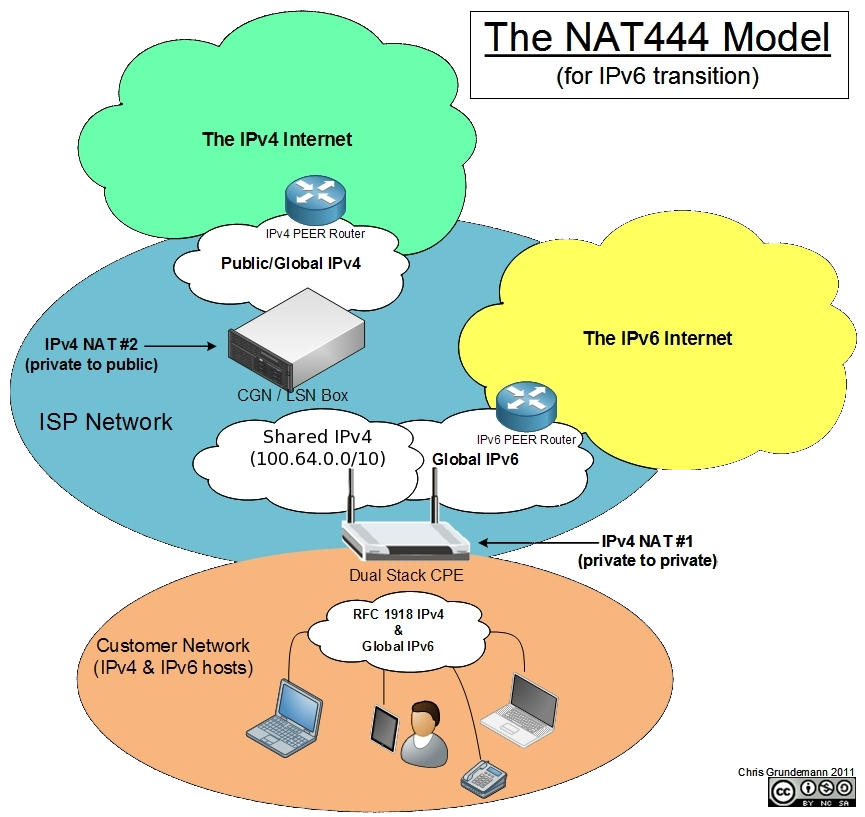
\includegraphics[width=\textwidth]{nat444.png}}
    \caption{esquema de uso do NAT444. Fonte:\cite{site:nat444}}
    \label{fig:nat444}
\end{figure}

\newpage
No \gls*{nat}444 \cite{site:nat444}, dois \glspl*{nat} são usados, e é possível
perceber que:

\begin{itemize}
    \item \gls*{nat}444 de IPv4 funcionando em pilha dupla (\emph{dual stacked}; para
        ambos os protocolos) com IPv6 global (público); e

    \item \gls*{nat}444 adiciona uma segunda camada de \gls*{nat}, ou seja, uma segunda
        área de endereçamento ``interno'' (privada).
\end{itemize}

Ao adicionar a segunda camada, vários usuários podem ter um mesmo endereço, ou seja, o
\gls*{isp} deverá tomar medidas de como registrar os acessos com as respectivas portas
de entrada e saída, por questões legais. Outro fato é que deve-se aceitar que o segundo
\gls*{nat} não será configurável por UPnP, por \gls*{nat}-PMP ou outros protocolos de
travessia de \gls*{nat}. Um \gls*{isp} não permitirá que ocorra essa configuração, pois
existirá o risco de um usuário afetar serviços de outros. Por esse motivo, é possível
prever aplicações que podem ser afetadas com problemas de desempenho, ou mesmo
incapacidade de execução \cite{site:rfcnat444}:

\begin{itemize}
    \item grandes downloads por FTP;
    \item \emph{seeding} em Limewire e BitTorrent;
    \item jogos online (Xbox, Playstation, etc);
    \item \emph{streaming} de vídeo (Hulu, Netflix, etc);
    \item acesso remoto de webcam;
    \item tunelamento para IPv6 (6to4, Teredo, etc);
    \item VPN e criptografia (IPSec, SSL);
    \item VoIP.
\end{itemize}